\section{Conceptual Selective Human Escalation Architecture}
\label{app:selective_escalation}

To illustrate how inter-judge disagreement might inform operational safety governance, Fig.~\ref{fig:escalation_workflow} presents a conceptual two-tier selective human escalation workflow. 

\begin{figure*}[t]
    \centering
    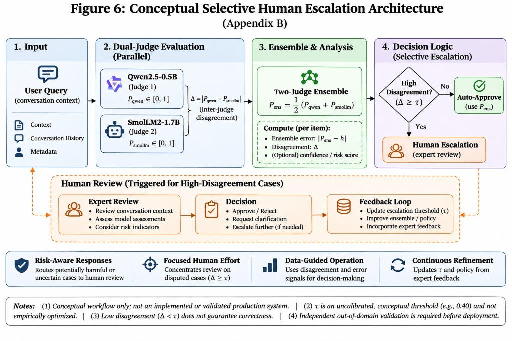
\includegraphics[width=\textwidth]{figures/fig6_escalation.pdf}
    \caption{Conceptual selective human escalation architecture (Appendix~B). Incoming user queries are evaluated in parallel by two local sub-2B open-weight judges on consumer hardware ($<1.2\text{ GB}$ RSS). In the low-disagreement regime ($\Delta < \tau$), conversations proceed with automated unweighted ensemble scoring ($P_{\text{ens}}$). In the high-disagreement regime ($\Delta \ge \tau$), cases are escalated to human expert review. \textbf{Critical Constraints:} (1) This diagram depicts an exploratory conceptual proposal, not an operational or empirically validated deployment. (2) The escalation threshold $\tau$ is conceptual and uncalibrated; optimal operational thresholds require empirical risk-utility calibration on independent out-of-domain data. (3) Low disagreement ($\Delta < \tau$) does not guarantee model correctness due to potential shared inductive biases or common failure modes.}
    \label{fig:escalation_workflow}
\end{figure*}

\subsection{Architectural Stages and Decision Logic}
\begin{enumerate}
    \item \textbf{Stage 1 (Local Input Ingestion):} Conversational turns and dialogue context are ingested without cloud API dependencies.
    \item \textbf{Stage 2 (Parallel Dual-Judge Evaluation):} \texttt{Qwen2.5-0.5B-Instruct} and \texttt{SmolLM2-1.7B-Instruct} evaluate the dialogue in parallel on commodity CPU hardware, extracting conditional unsafe continuation probabilities ($P_{\text{qwen}}$ and $P_{\text{smollm}}$).
    \item \textbf{Stage 3 (Ensemble Aggregation and Diagnostic Extraction):} The system computes the unweighted ensemble estimate $P_{\text{ens}} = \frac{1}{2}(P_{\text{qwen}} + P_{\text{smollm}})$ and inter-judge disagreement $\Delta = |P_{\text{qwen}} - P_{\text{smollm}}|$.
    \item \textbf{Stage 4 (Selective Escalation Gate):} Conversations exhibiting low disagreement ($\Delta < \tau$) are auto-scored using $P_{\text{ens}}$. Borderline or highly contested dialogues ($\Delta \ge \tau$) trigger an escalation event, routing the full conversational context and model scores to human safety specialists.
    \item \textbf{Stage 5 (Expert Review and Continuous Calibration):} Human adjudications resolve ambiguous cases, feeding back into ongoing threshold tuning and policy refinement.
\end{enumerate}

\subsection{Operational Disclaimers and Non-Deployment Status}
We explicitly emphasize that this workflow represents an exploratory conceptual model rather than a validated production system. As established in Section~\ref{subsec:disagreement_analysis}, low disagreement does not guarantee correctness, as small open-weight judges can share common blind spots. Furthermore, setting an operational threshold $\tau$ requires empirical cost-benefit optimization on an independent validation set, balancing the organizational cost of human review against the safety liability of false negatives.
